\chapter{La superficie stradale}
\label{rdf}
%
Oltre allo pneumatico, la superficie stradale rappresenta il secondo importante elemento che definisce il contatto. Perché una superficie stradale possa essere facilmente utilizzata da un calcolatore deve essere prima discretizzata. La discretizzazione in questo caso avviene mediante la rappresentazione della superficie stessa in una \textit{mesh} triangolare. La \textit{mesh} è contenuta in un \textit{file} di formato \ac{RDF}, che contiene le posizioni $(x,y,z)$ di ogni vertice e i numeri di identificazione per ognuno dei tre vertici del triangolo, per ogni triangolo.\\
\indent
È importante notare che la discretizzazione del manto stradale è un processo molto importante in quanto, se campionato troppo grossolanamente potrebbe influire negativamente sui risultati dei calcoli per l'estrazione del piano strada locale. In altre parole, una semplificazione eccessiva, potrebbe causare degli errori tali da incorrere in risultati troppo approssimativi e non rispecchianti la realtà. Al contrario, una \textit{mesh} troppo fitta, aumenterebbe inutilmente i calcoli da eseguire, dilatando quindi i tempi di esecuzione. È bene quindi discretizzare più densamente in maniera oculata e solo dove occorre realmente, ovvero in prossimità di cordoli, marciapiedi o qualsiasi tipo di ostacolo che potrebbe influire sulle prestazioni della vettura.

\section{Il formato RDF}
%
\subsection{Superfici semplici}
Sfortunatamente, non esistono \textit{standard} universalmente riconosciuti per il formato RDF. In linea di massima le superfici stradali sono definite nei \textit{Road Data File} (\texttt{*.rdf}). Questa tipologia di \textit{file} è composta da varie sezioni, indicate da parentesi quadre.
\begin{pseudoc}
	{ Comments section }
	
	[UNITS]
	LENGTH = 'meter'
	ANGLE = 'degree'
	
	[MODEL]
	ROAD\_TYPE = '...'
	
	[PARAMETERS]
	...
\end{pseudoc}
Nella sezione \texttt{[UNITS]}, vengono impostate le unità di misura utilizzate nel \textit{file}. La sezione \texttt{[MODEL]} viene invece utilizzata per specificare la morfologia della superfice stradale, che può essere del tipo:
\begin{itemize}
	\item \texttt{ROAD\_TYPE = 'flat'}: superficie stradale piana.
	\item \texttt{ROAD\_TYPE = 'plank'}: singolo scalino o dosso orientato perpendicolarmente o obliquo rispetto all'asse $X$, con o senza bordi smussati.
	\item \texttt{ROAD\_TYPE = 'poly\_line'}: altezza della strada è in funzione della distanza percorsa.
	\item \texttt{ROAD\_TYPE = 'sine'}: superficie stradale costituita da una o più onde sinusoidali con lunghezza d'onda costante.
\end{itemize}
La sezione \texttt{[PARAMETERS]} contiene i parametri generali e specifici per il tipo di superficie stradale. Possono essere:
\begin{itemize}
	\item Generali:
	\begin{itemize}
		\item \texttt{MU}: è il fattore di correzione dell'attrito stradale (non il valore dell'attrito stesso), da moltiplicare con i fattori di ridimensionamento \texttt{LMU} del modello di pneumatico.\\
		Impostazione predefinita: \texttt{MU = 1.0}.
		\item \texttt{OFFSET}: è l'offset verticale del terreno rispetto al sistema di riferimento inerziale.
		\item \texttt{ROTATION\_ANGLE\_XY\_PLANE}: è l'angolo di rotazione del piano $XY$ attorno all'asse $Z$ della strada, ovvero la definizione dell'asse $X$ positivo della strada rispetto al sistema di riferimento inerziale.
	\end{itemize}
	\item Strada con scalino:
	\begin{itemize}
		\item \texttt{HEIGHT}: altezza dello scalino.
		\item \texttt{START}: distanza lungo l'asse $X$ della strada dell'inizio dello scalino.
		\item \texttt{LENGTH}: lunghezza dello scalino (escluso lo smusso) lungo l'asse $X$ della strada.
		\item \texttt{BEVEL\_EDGE\_LENGTH}: lunghezza del bordo smussato a $45°$ dello scalino.
		\item \texttt{DIRECTION}: rotazione dello scalino attorno all'asse $Z$, rispetto all'asse $Y$ della strada.\\
		Se lo scalino è posizionato trasversalmente, \texttt{DIRECTION = 0}. Se lo scalino è posto lungo l'asse $X$, \texttt{DIRECTION = 90}.
	\end{itemize}
	\item Polilinea:\\
	Il blocco \texttt{[PARAMETERS]} deve avere un sotto blocco chiamato \texttt{(XZ\_DATA)} e costituito da tre colonne di dati numerici:
	\begin{itemize}
		\item La colonna 1 è un insieme di valori $X$ in ordine crescente.
		\item Le colonne 2 e 3 sono insiemi di rispettivi valori $Z$ per la traccia sinistra e destra.
	\end{itemize}
	Esempio:
	\begin{pseudoc}
	[PARAMETERS]
	MU = 1.0
	OFFSET = 0.0
	ROTATION_ANGLE_XY_PLANE = 0.0 
	
	{ X_road	Z_left	Z_right }
	(XZ_DATA)
	-1.0e04	0	0
	0.0500	0	0
	0.1000	0	0
	0.1500	0	0
	... ... ...
	\end{pseudoc}
	\item Sinusoide:\\
	La strada a superficie sinusoidale è implementata come:
	\begin{equation}
	z(x)=\frac{H}{2}\left( 1 - \cos \left( \frac{2\pi \cdot (x-x_i)}{L} \right)   \right) 
	\end{equation}
	dove	
	\begin{itemize}
	 	\item $z$: coordinata verticale della strada;
	 	\item $H$: altezza;
	 	\item $x$: posizione attuale;
	 	\item $x_i$: inizio dell'onda sinusoidale;
	 	\item $L$: semi-periodo dell'onda sinusoidale.
	\end{itemize}
	I parametri sono:	
	\begin{itemize}
		\item \texttt{HEIGHT}: altezza dell'onda sinusoidale.
		\item \texttt{START}: distanza lungo l'asse $X$ della strada dall'inizio dell'onda sinusoidale.
		\item \texttt{LENGTH}: lunghezza dell'onda sinusoidale lungo l'asse $X$ della strada.
		\item \texttt{DIRECTION}: rotazione dell'onda sinusoidale attorno all'asse $Z$, rispetto all'asse $Y$ della strada.\\
		Se l'onda sinusoidale è posizionata trasversalmente, \texttt{DIRECTION = 0}. Se l'onda sinusoidale è posta lungo l'asse $X$, \texttt{DIRECTION = 90}.
	\end{itemize}
\end{itemize}
%
\subsection{Superfici complesse}
Sfortunatamente, queste informazioni appena descritte permettono di costruire strade troppo semplicistiche e approssimative, che non rispecchiano la realtà. È quindi necessario inserire i risultati della discretizzazione della superficie stradale sopra citati.

Per descrivere la superficie stradale si utilizzerà dunque una \textit{mesh} poligonale. Quest'ultima può essere rappresentata utilizzando diversi metodi per memorizzare i dati dei vertici, bordi e facce. Nel caso specifico si andrà ad utilizzare una rappresentazione del tipo faccia-vertice. La \textit{mesh} faccia-vertice rappresenta un oggetto come un insieme di facce e un insieme di vertici. Questa rappresentazione è generalmente la più utilizzata in quanto permette una ricerca esplicita dei vertici di una faccia e delle facce che circondano un vertice.

Per descrivere una superficie stradale composta da una \textit{mesh} di triangoli si utilizzerà quindi la seguente struttura dati:
\begin{itemize}
	\item \texttt{[NODES]} (Vertici): presenti nella prima sezione, vengono descritti sotto forma di una quartina $(id,x,y,z)$ data dal numero di identificazione e dalle coordinate nello spazio.
	\item \texttt{[ELEMENTS]} (Facce): presenti nella seconda sezione, vengono descritti sotto forma di una quartina $(n_1,n_2,n_3,\mu)$ data dai numeri di identificazione dei tre vertici componenti $i$-esimo triangolo e dal coefficiente di attrito presente nella faccia.
\end{itemize}
Esempio:
\begin{pseudoc}
	[NODES]
	{ id x_coord y_coord z_coord }
	0 2.64637 35.8522 -1.59419e-005 
	1 4.54089 33.7705 -1.60766e-005 
	2 4.52126 35.8761 -1.62482e-005 
	3 2.66601 33.7456 -1.57714e-005 
	4 0.771484 35.8282 -1.56367e-005 
	5 0.791126 33.7206 -1.5465e-005
	... ... ... ...
	
	[ELEMENTS]
	{ n1 n2 n3 mu }
	1 2 3 1.0 
	2 1 4 1.0 
	5 4 1 1.0 
	... ... ... ...
\end{pseudoc}
Ulteriori parametri possono essere aggiunti prima della dichiarazione dei nodi della \textit{mesh}, come ad esempio:
\begin{itemize}
	\item \texttt{X\_SCALE}: riscala i punti delle coordinate dei nodi lungo l'asse $X$;
	\item \texttt{Y\_SCALE}: riscala i punti delle coordinate dei nodi lungo l'asse $Y$;
	\item \texttt{Z\_SCALE}: riscala i punti delle coordinate dei nodi lungo l'asse $Z$;
	\item \texttt{ORIGIN}: definisce la posizione dell'origine del sistema di riferimento della superficie stradale;
	\item \texttt{UP}: definisce la direzione positiva dell'asse $Z$;
	\item \texttt{[ORIENTATION]}: ruota i punti delle coordinate dei nodi secondo la matrice definita.
\end{itemize}
Esempio:
\begin{pseudoc}
	X_SCALE
	1000.0
	Y_SCALE
	1000.0
	Z_SCALE
	1000.0
	ORIGIN
	0 0 0
	UP
	0.0,0.0,1.0
	ORIENTATION
	1.0  0.0  0.0
	0.0  1.0  0.0
	0.0  0.0  1.0
\end{pseudoc}
%
\section{Analisi sintattico-grammaticale del formato RDF}
%
L'analisi sintattico-grammaticale è un processo che analizza un flusso continuo di dati in ingresso (letti per esempio da un \textit{file}) in modo da determinare la correttezza della sua struttura grazie ad una data grammatica formale. Il programma che esegue questo compito viene chiamato \textit{parser}. Nella maggior parte dei casi l'analisi sintattica opera su una sequenza di \textit{tokens} in cui l'analizzatore lessicale spezzetta l'\textit{input}.

Nel lavoro svolto è stato creato un algoritmo per eseguire l'analisi sintattico-grammaticale dei \textit{file} di tipo \ac{RDF}. Purtroppo, come precedentemente affermato, non esiste uno \textit{standard} universalmente riconosciuto per questo formato. Creare dunque un \textit{parser} o definire un generatore di \textit{parser} è arduo. Si è quindi optato per la creazione di un programma che rilevi solo i nodi (\texttt{[NODES]}), li salvi temporaneamente e, dopo aver immagazzinato anche i dati relativi agli elementi (\texttt{[ELEMENTS]}), istanzi un oggetto \textit{mesh}, composto dai nodi dichiarati nella sezione degli elementi. Gli altri parametri non sono stati considerati.

\begin{figure}
	\centering
	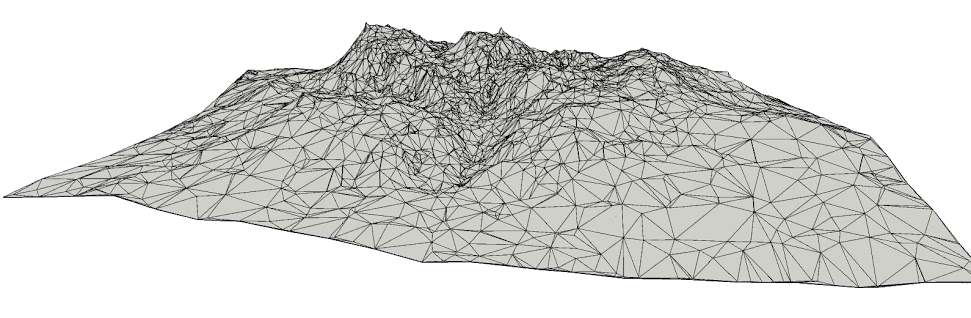
\includegraphics[width=0.7\linewidth]{Figures/mesh}
	\caption{Esempio di superficie rappresentata tramite \textit{mesh} triangolare.}
\end{figure}
\begin{figure}
	\centering
	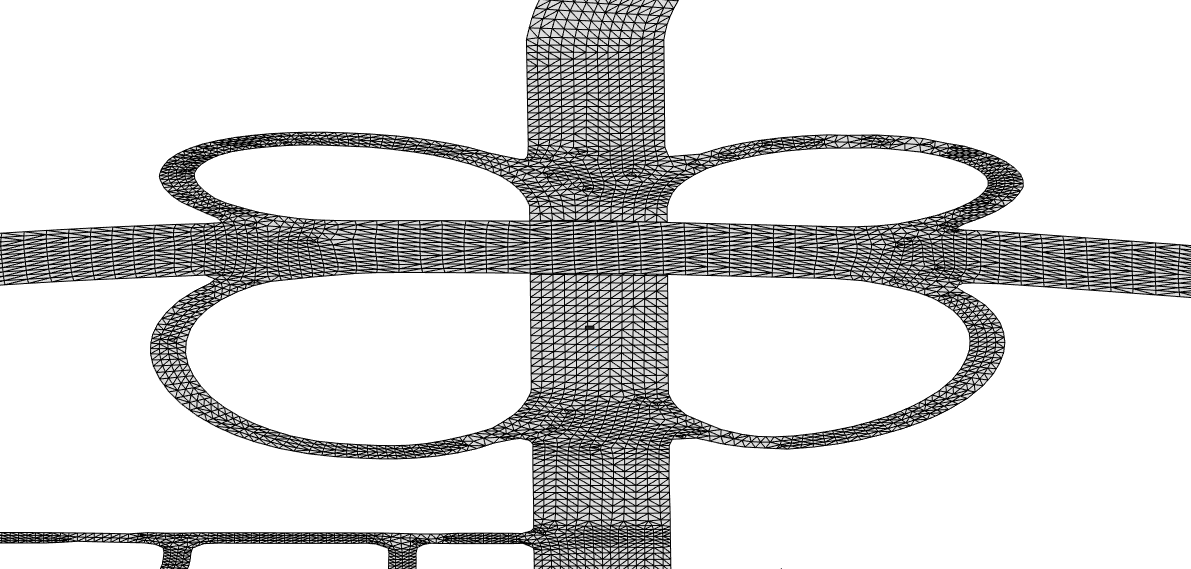
\includegraphics[width=0.7\linewidth]{Figures/mesh_1}
	\caption{Intersezione stradale rappresentata tramite \textit{mesh} triangolare.}
\end{figure}

Come verrà richiamato nelle conclusioni, l'importanza di definire uno \textit{standard} per il formato \ac{RDF} è di cruciale importanza. In questo modo si potrà creare un generatore di \textit{parser} con una grammatica e un lessico ben definiti, nonché aumentarne l'efficienza e la stabilità.